\documentclass[10pt,twocolumn,letterpaper]{article}
\usepackage{cvpr}
\usepackage{times}
\usepackage{epsfig}
\usepackage{graphicx}
\usepackage{amsmath}
\usepackage{amssymb}
\usepackage{mathtools} % mathtools builds on and extends amsmath package
\usepackage{algorithm}		% http://ctan.org/pkg/algorithms
\usepackage{algpseudocode}	% http://ctan.org/pkg/algorithmicx% Include other packages here, before hyperref.
\usepackage{comment, url}

% If you comment hyperref and then uncomment it, you should delete
% egpaper.aux before re-running latex.  (Or just hit 'q' on the first latex
% run, let it finish, and you should be clear).
\usepackage[pagebackref=true,breaklinks=true,letterpaper=true,colorlinks,bookmarks=false]{hyperref}

% \cvprfinalcopy % *** Uncomment this line for the final submission

\def\cvprPaperID{****} % *** Enter the CVPR Paper ID here
\def\httilde{\mbox{\tt\raisebox{-.5ex}{\symbol{126}}}}

% Pages are numbered in submission mode, and unnumbered in camera-ready
\ifcvprfinal\pagestyle{empty}\fi

\usepackage{color}

\newcommand{\matt}[1]{ \color{red} Matt: #1  \color{black}}
\newcommand{\aneesh}[1]{ \color{blue} Aneesh: #1  \color{black}}
\newcommand{\burak}[1]{ \color{green} Burak: #1  \color{black}}
\newcommand{\emmett}[1]{\color{violet} Emmett: #1  \color{black}}
\usepackage{forloop}
\newcounter{ct}
\newcommand{\markdent}[1]{\forloop{ct}{0}{\value{ct} < #1}{\hspace{\algorithmicindent}}}
\newcommand{\markcomment}[1]{\Statex\markdent{#1}}
\begin{document}


%%%%%%%%% TITLE
\title{ {\it E}nKCF: Ensemble of Kernelized Correlation Filters for Object Tracking in High Speed, 300Hz}

\author{Burak Uzkent\\
Rochester Institute of Technology\\
{\tt\small bxu2522@@rit.edu}
% For a paper whose authors are all at the same institution,
% omit the following lines up until the closing ``}''.
% Additional authors and addresses can be added with ``\and'',
% just like the second author.
% To save space, use either the email address or home page, not both
\and
YoungWoo Seo\\
Affiliation\\
{\tt\small youngwoo.blank.seo@gmail.com}
}

\maketitle
%\thispagestyle{empty}

%%%%%%%%% ABSTRACT
\begin{abstract}

\end{abstract}

%%%%%%%%% BODY TEXT
\section{Introduction}

\begin{comment}
Maybe the goal of this work is to publish a journal paper about a
practical solution for a drone to follow a single target. For this, we
need some descriptions on
\begin{itemize}
\item A vision-based, single target tracking algorithm.
\item Other components for making a drone follow a target.
\begin{itemize}
\item An architecture diagram
\item Descriptions of vehicle control, motion planning, behavior
  generation, estimation of relative geometry between a drone and a
  target, etc
\item Experimental results or example videos
\end{itemize}
\end{itemize}

For the BMVC-17 submission, we're going to just focus on the first
part -- a vision-based, single target tracking algorithm. This is
because we need to build a drone for the second part.
\end{comment}

\begin{itemize}
\item Introduction: Should talk about, at least, motivation of this
  work, brief review of the literature, and contribution
\item Method: Detail the method w.r.t. a diagram of system
  architecture or pseudo code
\begin{itemize}
\item Kernelized Correlation Filter
\item A variant of KCF: Multiple KCF w/ PF ({\it E}nKCF, ${\it E}nKCF_{+RD}$
\item Re-detection for re-initialization: Modules for reliably
  detecting target-lost, for extensively searching the lost target,
  and for picking up the same target with a help from an appearance
  model or other models.
\begin{itemize}
\item To filter out unlikely box proposals,
\begin{itemize}
\item Use a prior information about box, our outputs, dimensions
  (e.g., a combination of width and height, aspect ratio, etc.)
\item Use the information about the trajectory of the target before we
  lose the target.
\end{itemize}
\item MTH: revisited
\item To make a box tighter, generate our own box proposals based on
  the locations of top $k$ box proposals from object proposal methods,
  e.g., Edge Box.
\end{itemize}
\end{itemize}
\item Experiment: Detail the data, and experimental setup; results and findings
\item Will compare the performance of {\it E}nKCF, Naive{\it E}nKCF,
  ${\it E}nKCF_{+RD}$ with those of the following tracking methods.
\begin{itemize}
\item vanilla-KCF w/ a fixed scale,
\item vanilla-KCF w/ three different scales,
\item LCT (Long-term Correlation Tracking) \cite{ma2015long}: Temporal
  correlation of a target over frames; a pyramid for different scales;
  re-detection w/ an appearance classifier (i.e., a naive Bayes w/
  random fern features in combination of sliding window). Temporal
  context regressor for translation over significant deformation and
  target regressor for scale variation.
\item MEEM (Multiple Experts using Entropy Minimization)
  \cite{zhang2014meem}.
\item SAMF (Scale Adaptive KCF)
\item STC (fast tracking via Spatio-Temporal Context learning)
  \cite{zhang2014fast}: 
\item Struck (Structured Output Tracking with Kernels)
\end{itemize}
\begin{itemize}
\item Visual tracker benchmark (VTB)
\item DTB-70: w/ and w/o motion estimation,
\item UAV123 \footnote{A set of images acquired from an UAV is called
  ``UAV123'' and publicly available from
  https://ivul.kaust.edu.sa/Pages/Dataset-UAV123.aspx}
\item VOT
\end{itemize}
\item Conclusion
\end{itemize}

A proliferation of unmanned vehicle technologies has ever increased
interest on deployment of computer vision algorithms on embedded or
mobile platforms. For example, an unmanned air vehicle (UAV) equipped
with object or feature following would make it more useful in the
application of monitoring/surveillance/surveying on private
properties/wild-life/crop, video recording on sports/movies/events,
many others. In this paper, we propose an object tracking algorithm
that aims at running on any embedded or mobile platforms. In
particular,

{\it We may need to change this introductory sentence based on the
  results.}


The tracking-by-detection methods have recently used extensively as a
robust, powerful, and highly discriminative vision-based, object
tracking method replacing the preceding, generative object tracking
methods that primarily concerned about learning the appearance of the
target. 

The recent examples of the tracking-by-detection algorithms include
Tracking-Learning-Detection \cite{kalal2012tracking}, Multiple
Instance Learning \cite{babenko2009visual}, Correlation Filter based
trackers \cite{bolme2010visual,henriques2015high}, and Struck
\cite{hare2012efficient}. These tracking-by-detection methods learn
the model of the target's appearance on the fly while discriminating
the target from the background.

{\it Burak: It isn't clear what you're getting at here} Learning
an object-specific classifier in an online manner can better handle
challenging scenarios with the cost of increased complexity.

To train a (binary) classifier to detect the target at every frame,
the classifier needs positive and negative examples. In a typical set
up, a positive example is assumed to be given whereas a set of
negative examples can be randomly collected from the background around
the given positive example. Such a typical setup for a
tracking-by-detection method might have two issues related to its
performance: Firstly, the appearance of the randomly sampled negative
examples might be highly correlated with that of positive one,
resulting in ambiguous boundary between positive and negative
classes. Secondly for a real-time tracking, such a setup would not be
feasible for the practice because the number of training data
gradually increases. Due to these issues, most of the
tracking-by-detection methods focus on efficiently handling
incremental update of the learned classifier and on collecting a
small, but informative negative examples.

{\it Burak: Why do we even mention these issues? Is this somehow
  related to what we did for this paper?}

\begin{comment}
However, there can be two issues in this framework. First,
the randomly collected samples can have large correlation resulting in
a weak classifier. Also, such framework is not feasible for real-time
tracking as the number of samples gradually increases. Most of the
tracking-by-detection algorithms focus on efficient incremental update
of a classifier together with more useful background sampling.
\end{comment}

The workflow of our MKCF based long-term target following method can
be visualized in fig.~\ref{Workflow_figure}. Summarize what we discuss
in the next sections.
\begin{figure*}[!t]
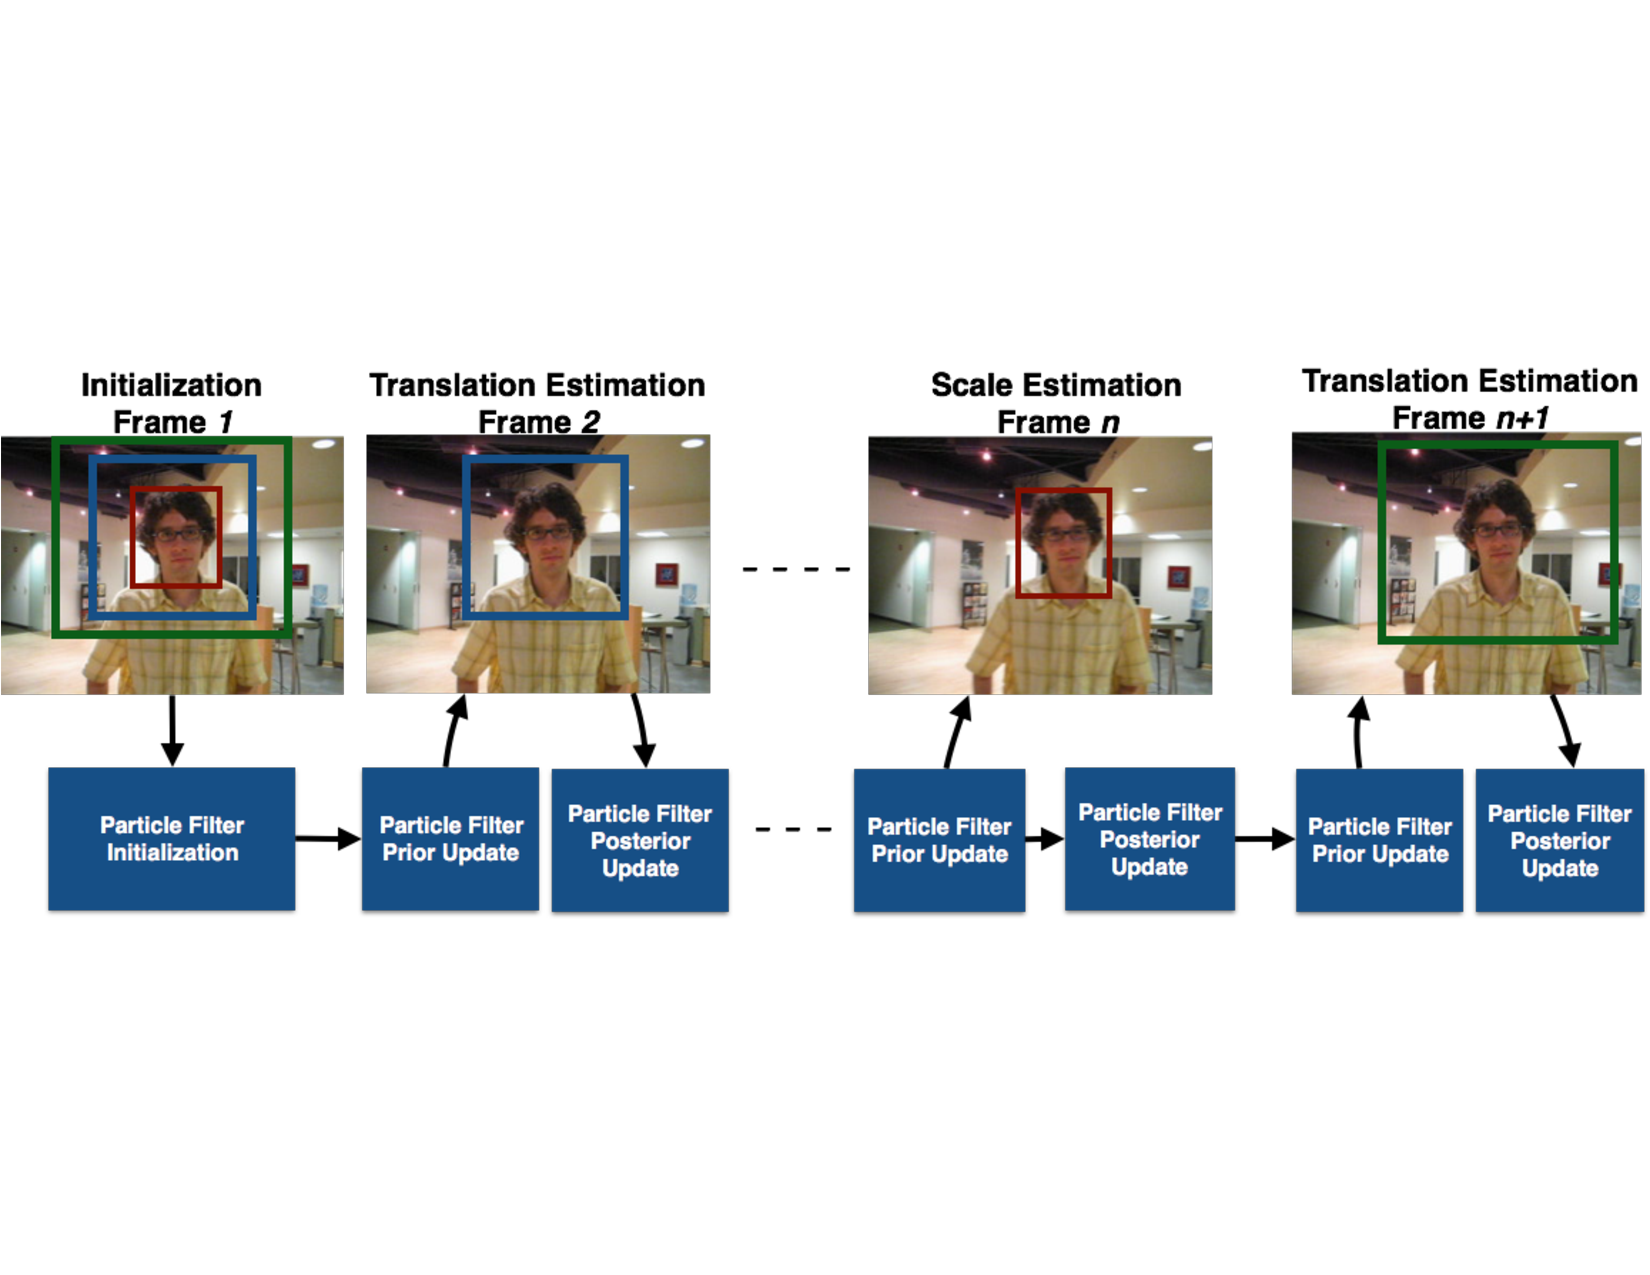
\includegraphics[width=\textwidth]{figures/Workflow_MKCF+PF.pdf}
\caption{The workflow of our Multiple KCF and Particle Filter based tracking method without the track re-detection module.}
\label{Workflow_figure}
\end{figure*}

An object tracking method based on the correlation filter in frequency
domain has gained attention due to its fast computation.

\begin{comment}
{\it Burak: This is not entirely true. If this is the case, people
  including us don't have to invent their own, other than just using
  KCF.}

Frequency domain correlation filter based trackers in the
tracking-by-detection paradigm has recently seen growing popularity
due to its superior computation and robustness to geometric and
photometric variations. 
\end{comment}

{\it YoungWoo: We'll have to mention why such an online tracker is
  still attractive over any DNN-based counterparts.}

To the best of our knowledge, the dominant framework of online object
trackers based on the correlation filter is to solve a regression
problem in the frequency domain. This framework assumes that the
target information is given at the very first image frame. Given this
positive example for the regression problem, a set of negative
examples is mostly collected around the initial, target bounding box
and represented as a circulant matrix \cite{henriques2015high}.

The first correlation filter tracker proposed by
\cite{bolme2010visual} focused on learning and detection in the
frequency domain. The idea was to minimize the sum of squared error in
the frequency domain. Hence, the convolution in the original domain is
avoided, instead, element-wise multiplication is needed in the
frequency domain. This way, it achieved promising performance at 700
Hz. On the other hand, the MOSSE tracker failed in cases with rapidly
changing background as it learns the filter using a single template
and accommodates single channel features. Later on, the MOSSE tracker
was improved by using the circularly shifted background patches in an
efficient way by utilizing the theorem that Discrete Fourier Transform
of a circulant matrix gives us diagonalized circulant matrix
\cite{henriques2012exploiting,henriques2015high}. In the same work,
the authors integrated kernelization concept into the detection and
learning steps to improve tracking
accuracy. \cite{galoogahi2013multi,henriques2015high} extended the
correlation filter trackers with single channel features to
multi-channel features. They employed the color and shape features in
a simple framework by summing the correlation of the test and learned
feature channels elements. There a few major drawbacks of the
correlation filter trackers although they outperformed the other
discriminative trackers with superior computation. First, due to the
nature of correlation filters it is limited to a region of interest
which is typically 2-3 times larger than the target. Considering a
larger ROI not only increases the computational burden but also leads
to further spatial information loss with the fixed template size. For
this reason, its performance degrades in fast motion cases as the ROI
may not contain the target. Second, the correlation filter lacks scale
adaptation ability since it only estimates the translation of the
target. Later studies focused on improving the latter issue by
proposing scale candidates where each scale is assigned a confidence
by performing detection on the shrinked or enlarged the ROI
\cite{li2014scale,tang2015multi,bibi2015multi,ma2015long}. Another
group of studies employ the part-based correlation filter trackers to
better adapt to the scale changes
\cite{liu2015real,akin2016deformable}. The sensitivity to fast motion
is generally handled in the long-term target tracking framework where
track reinilization module is triggered when the target is lost
\cite{ma2015long,de2015board,li2016monocular}.

The contributions of this study are as follows.
\begin{itemize}

\item \textbf{Single-Target Tracking in High-Speed} To be practical,
  the execution time of an object tracking is important. We proposed a
  new object tracking algorithm that is a collection of kernelized
  correlation filters (KCF). Each of KCFs is designed to address two
  challenges of object tracking: scale and translation. We also
  incorporate a Bayes filter to prevent from being drift.

\item \textbf{Re-Detection} A target loss is inevitable in object
  tracking. To cope with this, we developed a new target, re-detection
  that reliably detects when to lose the target and effectively
  re-detect the lost target. {\it How we can show how good our
    re-detection method is?}

\begin{comment}
\item We build a highly efficient ($\geq300$ fps) scale adaptive
  multiple kernelized correlation filter based tracker that
  outperforms the original KCF implementation with fixed scale
  framework both in terms of accuracy and performance. The studies
  following the KCF improved the fixed scale framework by running
  detection on a number of candidate ROIs to figure out the new scale
  of the object after estimating the translation of the object. This
  approach adds additional complexity to the original KCF
  implementation and drags down the run-time performance from $300$
  fps to less than $100$ fps.

\item We integrate the Particle Filter into the Multiple KCFs tracking
  as an additional filter that can avoid the drift due to one of the
  correlation filters we employ in our framework.

\item We propose a target re-detection module that can minimize the
  target loss due to the scale filter that learns the object model
  using only-object area. Also, the target re-detection step is
  required to handle severe occlusions, pose variations, illumination
  changes and fast motion.

\item Since our visual tracker mostly focuses on tracking objects from
  aerial moving platforms, we design a new robust target-to-camera
  distance estimation method. This way, a safe distance between the
  target and the camera-platform can be preserved.
\end{comment}

\end{itemize}

%---------------------------------------------------------------------- 
\section{{\it E}nKCF: Ensemble of Kernelized Correlation Filters}
%---------------------------------------------------------------------- 

% ---------------------------------------------------------
\subsection{Kernelized Correlation Filter Tracker} \label{KCF}
% ---------------------------------------------------------
The Kernelized Correlation Filter tracker has recently been
increasingly popular due to its operation at hundreds of frames per
second with state-of-the-art tracking capabilities in challenging
cases. Its computational efficiency arises from its use of the
discrete fourier transform of the circulant matrix and frequency
domain element-wise operations knows hadamard product and
division. The first example of frequency domain trackers is the Linear
Correlation Filter tracker known as MOSSE tracker. It minimizes the
ridge regression function in the frequency domain using a single
template with continous desired gaussian response. The KCF tracker, on
the other hand, minimizes the regularized ridge regression function
shown below.
\begin{equation}
E(h) = \frac{1}{2}||y-\sum_{c=1}^{C}g*x_{c}||^{2} + \frac{\lambda}{2}\sum_{c=1}^{C}||h_{c}||^{2}
\label{eq:Closedform_RidgeReg}
\end{equation}
where $y$ represents the desired continous response whereas $h$ and
$x_{c}$ represents the learned correlation filter and training
template for the given channel. The $c$ parameter included in
\cite{henriques2015high,galoogahi2013multi} makes it possible to
integrate multi-channel features such as HoG and colour into the ridge
regression function. The closed-form solution for the
eq.~\ref{eq:Closedform_RidgeReg} can be obtained by setting the
derivative of $E$ w.r.t $w$ to $0$. The solution in the primal domain
can be formulated as
\begin{equation}
w = (X^{T}X+\lambda)^{-1}y
\label{eq:SpatialSolution}
\end{equation}
where $X$ and $\lambda$ represent the training samples and
regularization term. The same cost function in the Fourier domain can
be represented as
\begin{equation}
w = (X^{H}X+\lambda I)^{-1}X^{T}y
\label{eq:FourierSolution}
\end{equation}
More information on the spatial and fourier domain solutions can be
found in \cite{henriques2015high}. The MOSSE tracker does not make use
of $\lambda$ and only one training sample with desired response is
used to update $w$. This framework does not include enough background
information into the training framework with a single template. The
application of the circulant matrix theorem into the
eq.~\ref{eq:Closedform_RidgeReg} makes it possible to include many
background patches at a similar computational complexity. A circulant
matrix $C$ includes the circularly shifted patches of the positive
training sample $x$ by the cylic shift operator $P$. By applying
shifting operation to the base sample, we can generate the circulant
matrix as
\begin{equation}
C = Px.
\label{eq:CirculantMatrixGeneration}
\end{equation}
The circulant matrix of a base sample $x$ can be interpreted as the
rows of a training matrix $X$ where each row represents features of a
training sample. Mathematically, this can be written as
\begin{equation}
X = C(x)
\label{eq:CIrculantMatrixTrainingData}
\end{equation}
In this form, eq.~\ref{eq:SpatialSolution}
and~\ref{eq:FourierSolution} could prohibit us from implementing a
high speed object tracking as we need to perform large number of
element-wise division and multiplication operations. However, we know
from \cite{gray2006toeplitz} that all circulant matrices are
represented diagonally by the Fourier Transform regardless of the base
sample $x$ as shown below.
\begin{equation}
X = Fdiag(\hat{x})F^{H}.
\label{eq:CirculantMatrixDFT}
\end{equation}
where $F$ denotes a constant Fourier Transform matrix and $x$ is the
Discrete Fourier Transform of the base sample $x$. To simplify the
cost function formulation in eq.~\ref{eq:FourierSolution} we multiply
$X$ in eq.~\ref{eq:CirculantMatrixDFT} with $X^{H}$ yielding
\begin{equation}
X^{H}X = Fdiag(\hat{x}^{*}\odot \hat{x})F^{H}.
\label{eq:SimplificationX} 
\end{equation}
Finally, the eq.~\ref{eq:SimplificationX} can used to formulate the
solution vector in Fourier domain $\hat{w}$ as
\begin{equation}
\hat{w} = \dfrac{\hat{x}^{*}*\hat{y}}{\hat{x}^{*}*\hat{x}+\lambda}.
\label{eq:DiagonalizedPrimalSolution}
\end{equation}
For detailed documentation of the circulant matrix theorem based
frequency domain solution can be found in
\cite{henriques2012exploiting,henriques2015high}.

The above primal frequency domain solution can be called as Linear
Correlation Filter which improves the MOSSE tracker by incorporating
cyclic shifts and regularizer. To further improve the robustness to
geometric and photographic variations, one can exploit non-linear
regression function in the Correlation Filter framework
\cite{henriques2015high}. The solution to the kernelized ridge
regression function is shown below.
\begin{equation}
\alpha = y(K+\lambda I)^{-1}
\end{equation}
wjere $K$ and $\alpha$ represent the kernel matrix and corresponding
dual space solution. \cite{henriques2015high} states that kernel
matrices is circulant for datasets of circular cylic satisfying the
following theorem.
\begin{equation}
k(x,x^{'}) = k(Mx,Mx^{'})
\label{eq:KernelCirculantTheorem}
\end{equation}
where $M$ represents the permutation matrix. Some kernels satisfying
the eq.~\ref{eq:KernelCirculantTheorem} are \textit{Gaussian},
\textit{Polynomial}, \textit{Intersection} and \textit{Hellinger}
kernels. Similar to the diagonalization in the linear ridge regression
solution in eq.~\ref{eq:DiagonalizedPrimalSolution}, the kernelized
ridge regression can be made diagonal using the same circulant matrix
theorem.  The diagonalized Fourier domain dual form solution can be
expressed as
\begin{equation}
\hat{\alpha} = \hat{y}(\hat{k}^{xx}+\lambda)^{-1}
\label{eq:FourierDualDomainSolution}.
\end{equation}
where $\hat{k}^{xx}$ represents the first row of the Kernel matrix $K$
known as \textit{gram matrix}. In this study, we will only focus on
application of the Gaussian Kernel to the Correlation Filters. We
refer the readers to \cite{henriques2015high} for the detailed
documentation of the application of other kernels to the Correlation
Filters. For single channel features, the Gaussian kernelization is
expressed as
\begin{equation}
k^{xx^{'}} = exp(-\dfrac{1}{\alpha^{2}}(||x||^{2}+||x^{'}||^{2}-2F^{-1}(\hat{x}^{*}\odot \hat{x}^{'})))
\label{eq:GaussianCorrelationSingleChannel}
\end{equation}
The first correlation filter based trackers used grayscale feature to
learn the solution vector $w$, however, the multi-channel features
such as HoG and Color were later exploited to improve tracking
accuracy
\cite{henriques2015high,galoogahi2013multi,tang2015multi,ma2015long,bibi2015multi}. The
multi-channel feature integration into the Gaussian Kernelization
function in eq.~\ref{eq:GaussianCorrelationSingleChannel} is achieved
in a very straight-forward way by summing the correlation result in
all the channels as
\begin{equation}
k^{xx^{'}} = exp(-\dfrac{1}{\alpha^{2}}(||x||^{2}+||x^{'}||^{2}-2F^{-1}(\sum^{C}_{c}\hat{x}_{c}^{*}\odot \hat{x}_{c}^{'}))).
\label{eq:GaussianCorrelationSingleChannel}
\end{equation}
Such non-linearization process does not increase the computational
complexity of the linear multi-channel correlation filter dramatically
as we only need to sum over the $n$ dimensional feature
channels. Training shown in eq:~\ref{eq:FourierDualDomainSolution}
gives us $\hat{a}$ learned in time step $t$. We can accumulate
$\hat{a}$ over time to integrate more temporal information. This can
be expressed as
\begin{equation}
\hat{a}_{t} = (1-\beta)\hat{a}_{t-1} + \beta\hat{a}_{t}. 
\end{equation}

Finally, detection step in multi-channel KCF framework is performed as
\begin{equation}
r(z) = F^{-1}(\hat{k}^{xz} \odot \hat{\alpha})
\end{equation}
where $r$ denotes the correlation response at all cylic shifts of the
first row of the kernel matrix $K$. The peak point of the response
function gives us the estimated translation of the object from time
step $t$-$1$ to $t$.

%-------------------------------------------------------------------
\subsection{Multiple Kernelized Correlation Filter Based Tracking} \label{sc:MKCF}
%------------------------------------------------------------------
The KCF with Multi-channel features outperforms the other
state-of-the-art object traking algorithms both in terms of run-time
performance and tracking accuracy. However, it lack scale adaptation
module or the naive scale adaptation method added into the KCF reduces
the frames per second from $\geq300$ fps to less than $100$ fps. One
straightforward method is to run detection on ROIs with different
sizes determined by pre-defined scale ratios
\cite{henriques2015high,tang2015multi,ma2015long,bibi2015multi,li2014scale}. All
these method increases the computational complexity of tracking by
running detection on a number of ROIs. Another scale update method in
Correlation Filter framework was proposed by \cite{zhang2014fast}. It
uses the MOSSE tracker to estimate translation of an object. The scale
is updated in a naive way where the confidence map is used to
determine the scale change between successive frames. For instance,
their method assumes similar scale in between two consecutive frames
given similar confidences. With this simple method, we do not need to
run detection on different ROIs at a given frame and perform tracking
at $\geq300$ fps. In this study, we propose the use of Multiple KCFs
in an intuitive way to perform robust scale-adaptive tracking at more
than $300$ fps. Our approach is inspired by \cite{ma2015long} where
two KCFs are employed as translation and scale filters. It first
estimates translation using the translation filter learned on
\textit{target}$+$\textit{background} area. Then, the scale filter
learned on the \textit{target} area is used to estimate new scale of
the target at the estimated position. Application of translation and
scale filter at each frame reduces run-time performance ($\leq50 fps$)
as we need to run detection and training on both filters. Similarly,
we learn three different correlation filters specializing on different
aspects of tracking and addresses the weakness of each other,
resulting in more robust tracking. We name these filters as
\textit{target}+\textit{small background} translation filter
($R_{t}^{S}$), \textit{target-only} scale filter ($R_{s}$) and
\textit{target}+\textit{large background} translation filter
($R_{t}^{L}$). Unlike \cite{ma2015long}, by running a single filter at
each frame, we can achieve the targeted operation frame rate. The
fig.~\ref{fig:Filters} shows the size of the ROIs associated with
$R_{t}^{S}$, $R_{t}^{L}$, and $R_{s}$ in addition to the hanning
windows assigned and desired Gaussian responses assigned to each one.

\begin{figure}[!t]
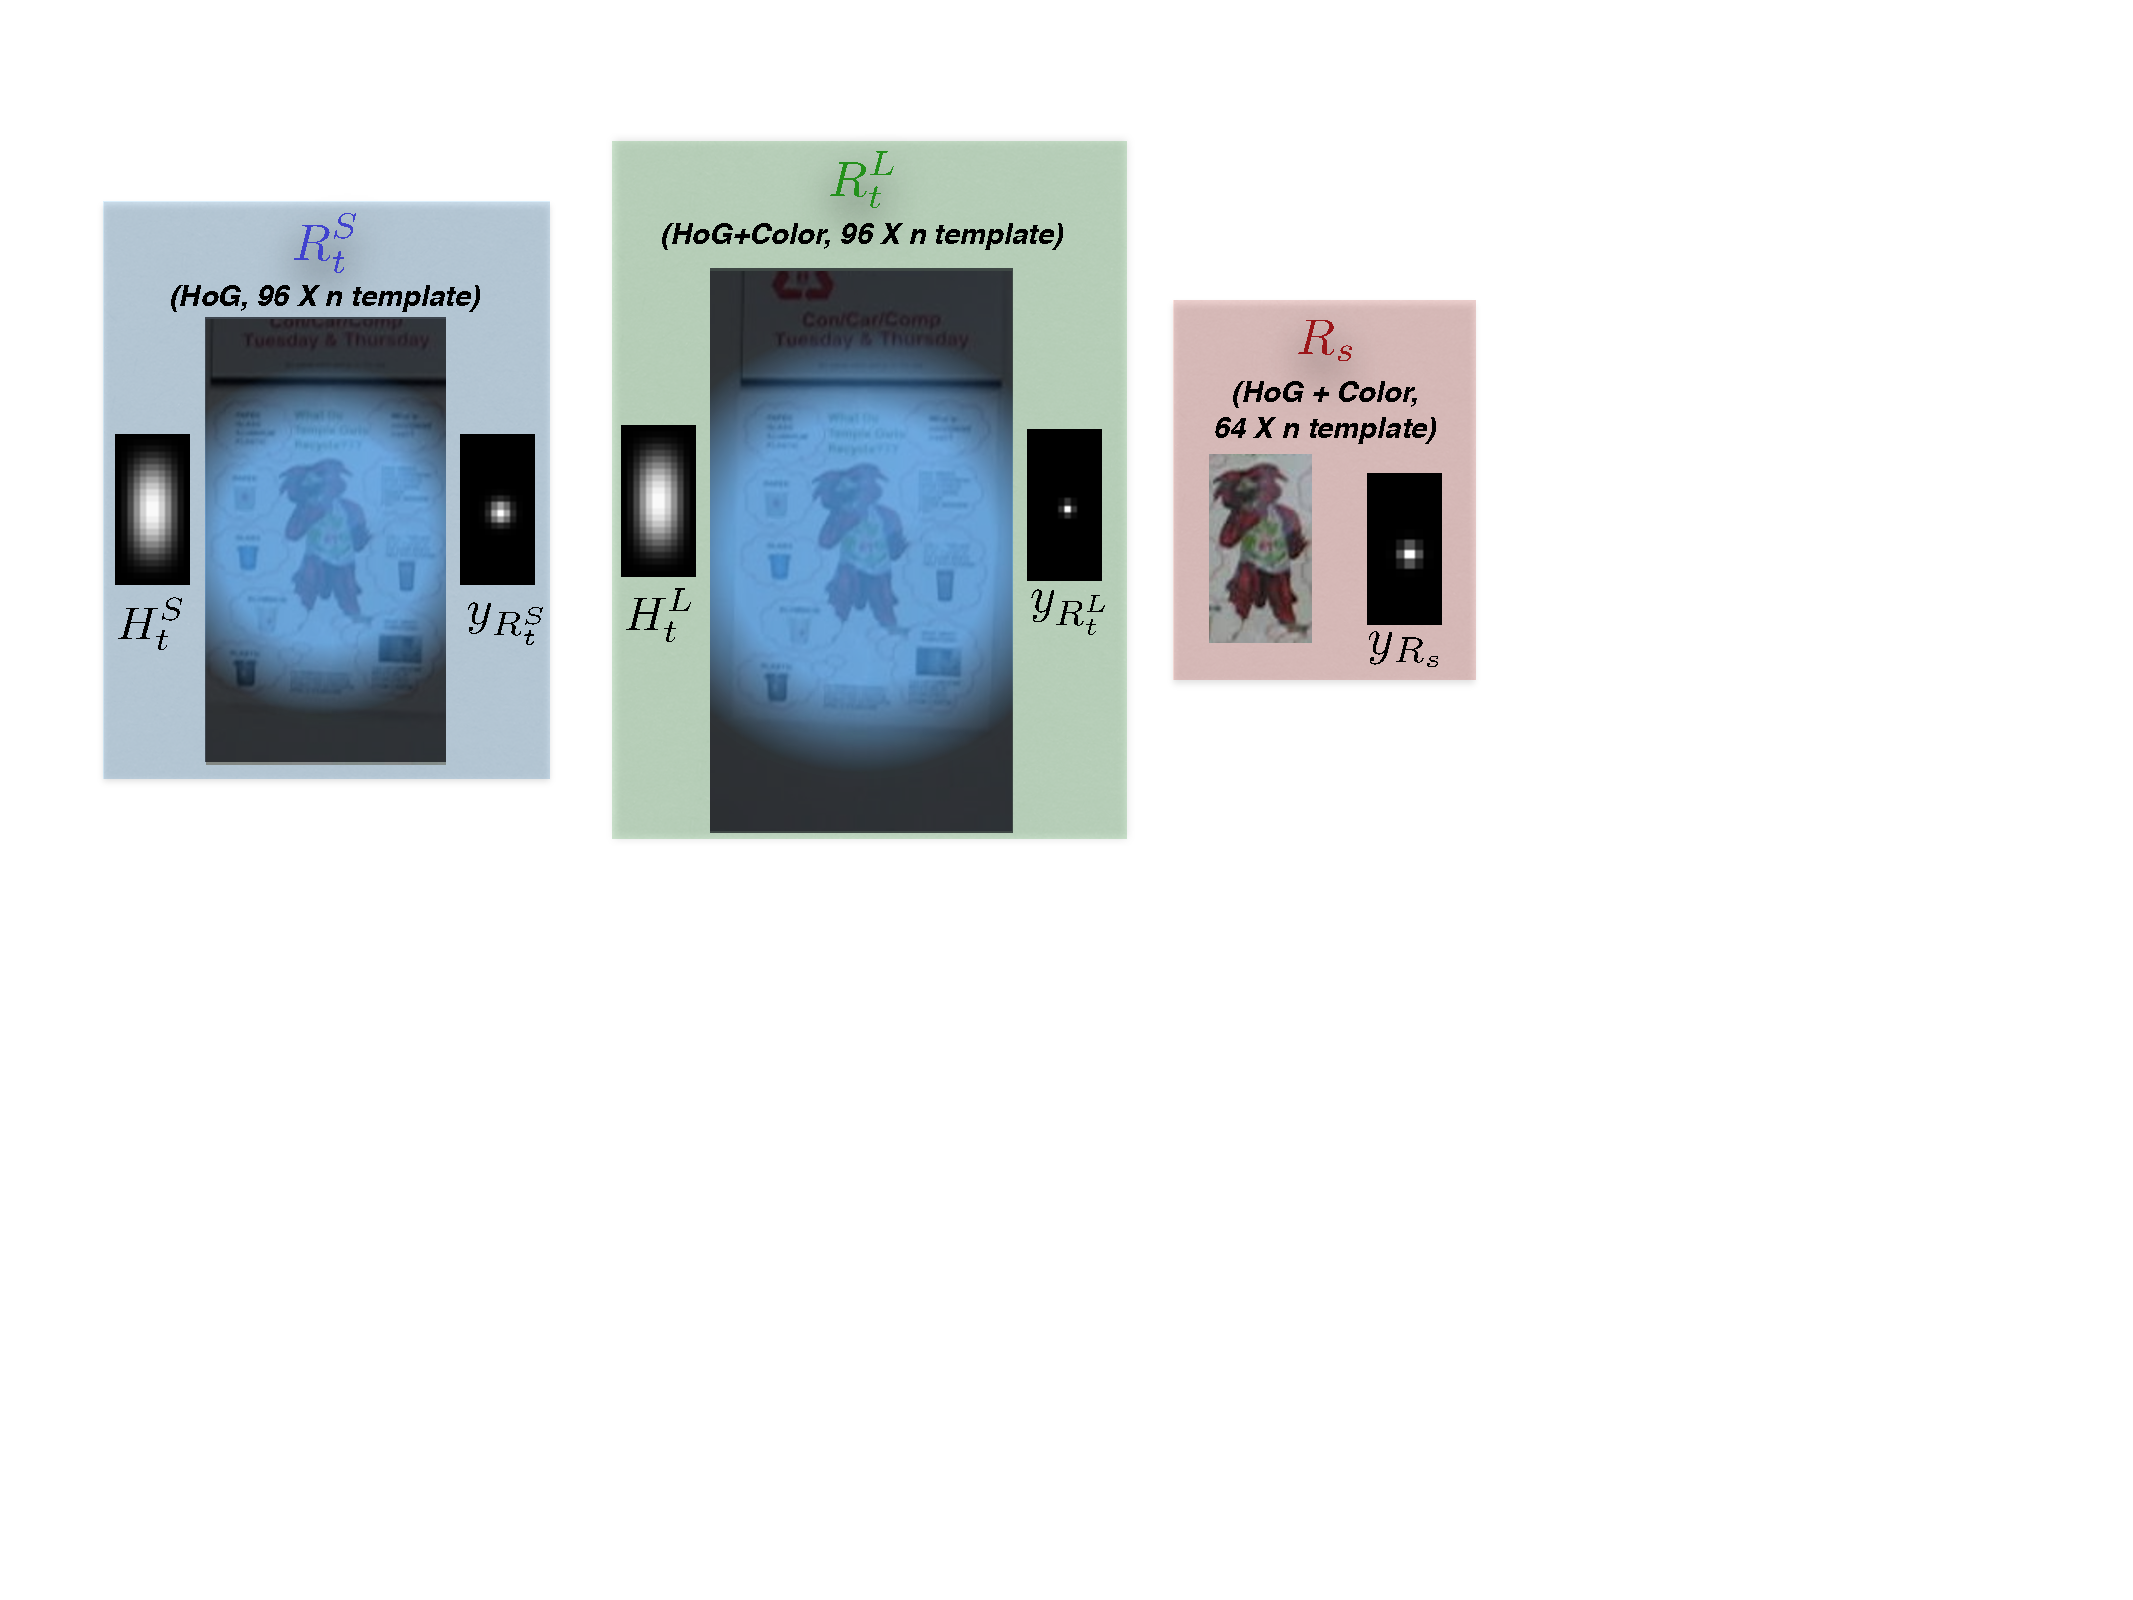
\includegraphics[width=0.5\textwidth]{figures/Filters_Details.pdf}
\caption{The three filters called as medium ROI translation filter,
  target ROI scale filter and large ROI translation filter are
  shown. Also, the hanning window and desired Gaussian response for
  each filter are displayed.}
\label{fig:Filters}
\end{figure}

Our MKCF based tracking framework employs different capabilities and
tasks to each correlation filter learned temporally. In
\cite{ma2015long, danelljan2014accurate}, a scale filter is learned on
\textit{target-only} area whereas \cite{henriques2015high,
  li2014scale, bibi2015multi, tang2015multi} uses a correlation filter
learned on \textit{target+background} area to find the optimal scale
in scale space. To learn the scale filter, $R_{s}$, we follow a
similar approach to \cite{ma2015long}. We believe that translation
filter needs to include background information to better discriminate
target from background, however, the goal of the scale filter is to
estimate the right size of the target, not to discriminate it from
background. Also, by using a smaller ROI we can reduce the size of the
template to learn the scale filter, resulting in higher speed scale
estimation module. Finally, the scale filter help us on the track
re-initialization module which includes running an object proposals
algorithm to boxes bounding the objects in the scene. By using the
scale filter in re-initialization module, we can reduce the
element-wise operations compared to the translation filters. The
\textit{target+small background} area translation filter, $R_{t}^{S}$,
is assigned a larger template size than $R_{s}$ and smaller than
$R_{t}^{L}$. It is employed to estimate translation and scale similar
to \cite{henriques2015high}. Finally, the \textit{target+large
  background} area translation filter, $R_{t}^{L}$ , estimates only
the translation of a target.

\begin{algorithm}
	\caption{The MKCF Tracking Algorithm.}\label{alg:MKCF}
	\begin{algorithmic}[1]
	\State \textbf{Input} : Initial bounding box $x_{0}$, frame counter $fc$, scale filter frequency $n$,
	\State \textbf{Output} : 
				\If{$fc\:\%\:n=0$} \Comment{Condition 1}
						\State Estimated Target State $x_{t} = (x_{t-1},y_{t-1},s_{t})$,
						Scale filter (\textit{target-only}) model $R_{s}$.
			     \EndIf
				\If{$fc\:\%\:n=1$}\Comment{Condition 2}
						\State Estimated Target State $x_{t} = (x_{t},y_{t},s_{t_1})$,
						Large Area Translation Filter model $R_{t}^{L}$.
				\EndIf
				\If{$fc\:\%\:n>1$}\Comment{Condition 3}
						\State Estimated Target State $x_{t} = (x_{t},y_{t},s_{t})$,
						Small Area Translation Filter model $R_{t}^{S}$.
				\EndIf
	\Procedure{track}{$x_{t-1},y_{t-1},s_{t-1}$} 
				\State // Translation Estimation
				\State Transit Particle Filter to the frame $t$ and compute the mean of prior pdf $x_{t} = (x_{t},y_{t},s_{t-1})$;
				\State // Translation Estimation
				\State Crop the ROI for the $R_{t}^{L}$, or $R_{t}^{S}$ given $x_{t}$
				and estimate translation ($x_{t}$,$y_{t}$) using $R_{t}^{L}$ (Condition 2) or $R_{t}^{S}$ (Condition 3),
				\State Skip translation estimation for $R_{s}$ (Condition 1);
				\State // Scale Estimation
			    \State Crop the ROI for the $R_{s}$ and estimate scale, $s_{t}$, using $R_{s}$ (Condition 1) or $R_{t}^{S}$ (Condition 2), 
		         \State Skip it for $R_{t}^{L}$ (Condition 1),
				\State Scale pool for $R_{s}$ : $\lbrace1.05,1.0,1/1.05\rbrace$, and for $R_{t}^{S}$ : $\lbrace1.02,1.0,1/1.02\rbrace$;
				\State // Update Translation
				\State Perform Importance Re-sampling for Particle Filter and compute the mean of posterior pdf $x_{t} = (x_{t},y_{t},s_{t})$;
			    \State // Model Update
				\If{$max(y_{R_{s}}) \geq T_{R_{s}}$}
				\State Update $R_{s}$ (Condition 1);
				\EndIf							 
				\If{$max(y_{R_{t}^{L}}) \geq T_{R_{t}^{L}}$} 
				\State Update $R_{t}^{L}$ (Condition 2);
				\EndIf	
			     \If{$max(y_{R_{t}^{S}}) \geq T_{R_{t}^{S}}$}
				\State Update $R_{t}^{S}$ (Condition 3);
			     \EndIf		
	\EndProcedure	
	\end{algorithmic}
\end{algorithm}

\section{Particle Filter}
\label{sc:PF}
The proposed MKCF algorithm can cause undesired drift and noise in
tracking due to independent application of the correlation filters. To
mitigate the drift effect and reduce the noise, a Bayes Filter
representing the evolution of target's motion can be added into the
MKCF tracking framework. In this study, we consider a variant of a
Bayes Filter, \textit{Particle Filter}. The Particle Filter is a
Sequential Monte Carlo method that can approximate posterior
probability density functions (pdf) of a target motion. The
approximation becomes optimal with the infinite number of particles,
however, its run-time complexity grows exponentially with the number
of elements in the state space matrix, $X_{t}$. As the focus of this
study is to design a high speed tracker, we keep the number of state
space elements low and implement computationally cheap \textit{Weight
  Function} and \textit{Importance-Resampling} modules. We represent
the state space matrix as $X_{t} = \lbrace x,y,V_{x},V_{y}\rbrace$
where $x$ and $y$ are the centroid of the target and $V$ represents
the velocity components. We transit the particles with the well-known
first order Constant Velocity model. The centroid components are
applied Gaussian Noise whereas the velocity components are assigned
uniform noise representative of most of the objects. The observation
likelihood is modeled based on the confidence map of
$R_{t}^{L}$,$R_{t}^{S}$, and $R_{s}$. It can also be modeled based on
the euclidean distance between particle's centroid to the peak of the
confidence maps, however, we believe that the former approach could
result in further drifts in the case of multi-modal distributions. The
weights for the particles are computed with the bilinear interpolation
method.
\begin{equation}
	w_{p_{t}}(x_{t},y_{t}) = \dfrac{\splitfrac{y_{R}(x_{t}-1,y_{t}-1)+y_{R}(x_{t}+1,y_{t}+1)+}{y_{R}(x_{t}+1,y_{t}-1)+y_{R}(x_{t}-1,y_{t}+1)}}{4}
\end{equation}
where $w_{p}$ denotes the weight of the particle. The importance
re-sampling module is triggered when the number of effective particles
is smaller than a pre-defined threshold [Cite - Effective Number
  Samples Metric] to avoid variance getting too small. Re-sampling is
implemented with highly efficient low-variance ratio method
[cite]. Finally, the expected mean of the approximated posterior pdf
is computed as
\begin{equation}
	\hat{X}_{t} = \sum_{p=1}^{P}w_{p_{t}} X_{t}
\end{equation}

The particles are assigned equal weight ($\dfrac{1}{P}$) after the
importance re-sampling step. It should be emphasized that we skip
importance re-sampling step in the scale filter operation as the scale
filter contains \textit{target-only} area. In this case, the particles
outside of the scale filter ROI do not have weight correspondence in
the confidence map. Also, it is more likely to get noisy translation
estimation from the scale filter.

WE SHOULD ASSIGN THE PRIOR WEIGHTS TO EXPECTED MEAN ESTIMATION OF THE
POSTERIORS WHEN THE RE-SAMPLING IS SKIPPED.
\section{Track Re-initilization via Re-detection}
\label{sc:Re-initialization}

%\section{Geometry Estimation between Target and Drone}
%\label{sc:Geometry}

%----------------------------------------------------------------------
\section{Experiments} \label{sc:Experiments}
%---------------------------------------------------------------------- 
To verify the usefulness of our algorithm, we ran our algorithm using
three publicly available dataset:
VOT2015 \footnote{\url{http://www.votchallenge.net/}},
OTB100 \footnote{\url{http://cvlab.hanyang.ac.kr/tracker_benchmark/benchmark_v10.html}},
UAV123 \footnote{\url{https://ivul.kaust.edu.sa/Pages/Dataset-UAV123.aspx}}\cite{mueller2016uav123}.

%---------------------------------------------------------------------- 
\section{Conclusion} \label{sc:Conclusion}
%---------------------------------------------------------------------- 

%--------------
%\section*{Acknowledgements}
%put stuff here for the accepted , but not the ICCV version

\small
\bibliographystyle{ieee}
\bibliography{draft}

\end{document}
